\begin{figure}[htbp]
	\begin{minipage}[ht]{0.48\hsize}\centering
		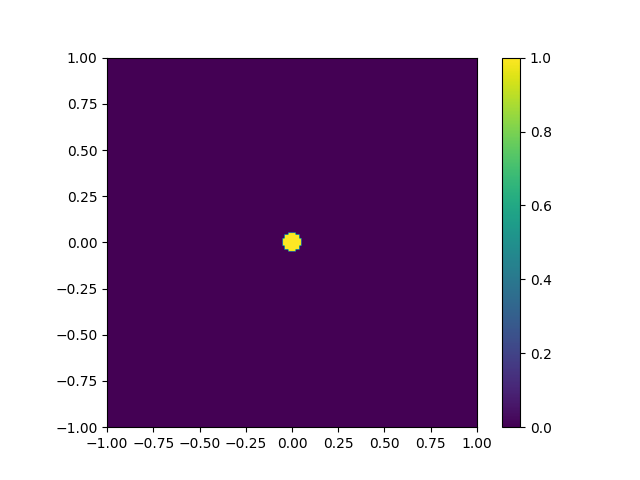
\includegraphics[width=\linewidth]{src/figures/result/circle1_original_estimation.png}
		\subcaption{円スリット (半径0.05)}\label{subfig:amplitude_sim_circle1_original}
	\end{minipage}
	\begin{minipage}[ht]{0.48\hsize}\centering
		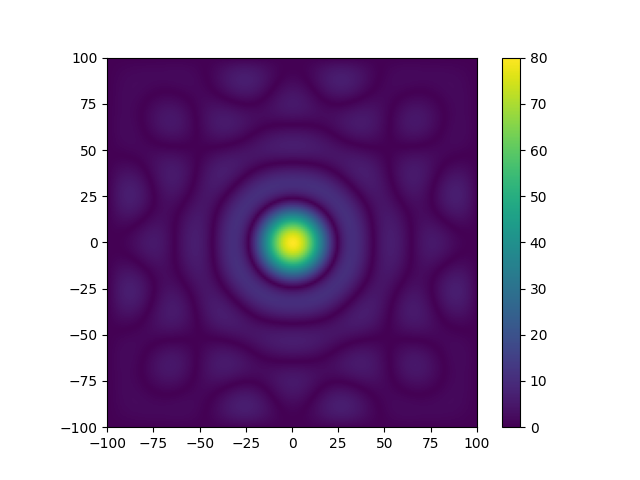
\includegraphics[width=\linewidth]{src/figures/result/circle1_amplitude_estimation.png}
		\subcaption{円スリット (半径0.05)の回折強度パターン}\label{subfig:amplitude_sim_circle1}
	\end{minipage}

	\begin{minipage}[ht]{0.48\hsize}\centering
		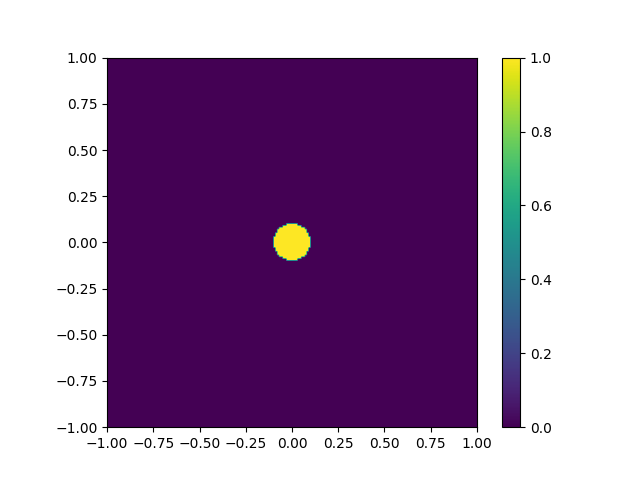
\includegraphics[width=\linewidth]{src/figures/result/circle2_original_estimation.png}
		\subcaption{円スリット (半径0.1)}\label{subfig:amplitude_sim_circle2_original}
	\end{minipage}
	\begin{minipage}[ht]{0.48\hsize}\centering
		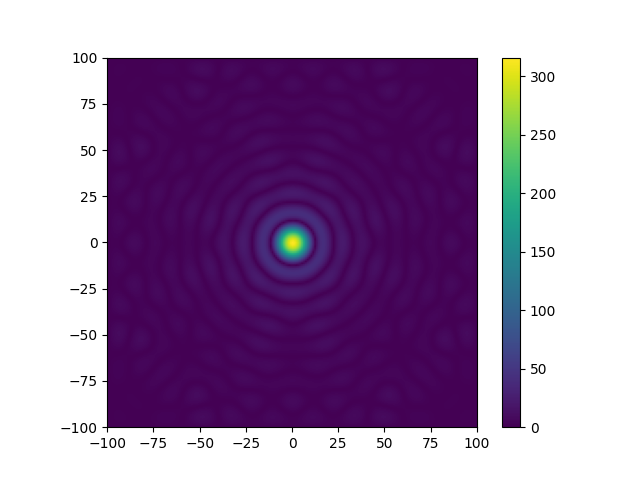
\includegraphics[width=\linewidth]{src/figures/result/circle2_amplitude_estimation.png}
		\subcaption{円スリット (半径0.1)の回折強度パターン}\label{subfig:amplitude_sim_circle2}
	\end{minipage}
	\caption{円スリットの回折強度パターンのシミュレーション}\label{fig:amplitude_sim_circle}
\end{figure}

\begin{figure}[htbp]
	\begin{minipage}[ht]{0.48\hsize}\centering
		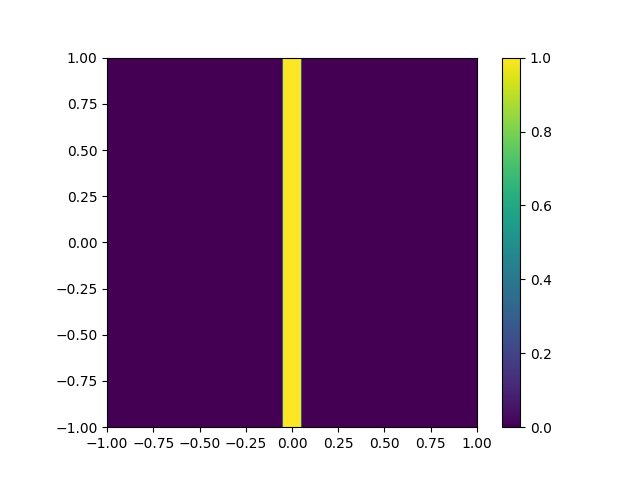
\includegraphics[width=\linewidth]{src/figures/result/ss1_original_estimation.png}
		\subcaption{単スリット (幅 0.05)}\label{subfig:amplitude_sim_single1_original}
	\end{minipage}
	\begin{minipage}[ht]{0.48\hsize}\centering
		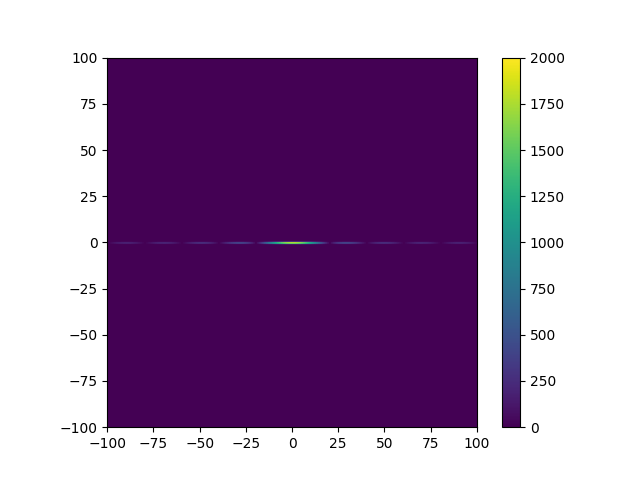
\includegraphics[width=\linewidth]{src/figures/result/ss1_amplitude_estimation.png}
		\subcaption{単スリット (幅 0.05)の回折強度パターン}\label{subfig:amplitude_sim_single1}
	\end{minipage}
	\begin{minipage}[ht]{0.48\hsize}\centering
		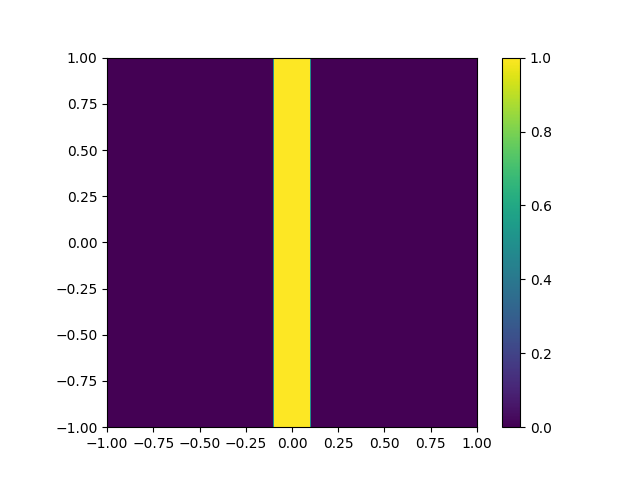
\includegraphics[width=\linewidth]{src/figures/result/ss2_original_estimation.png}
		\subcaption{単スリット (幅 0.1)}\label{subfig:amplitude_sim_single2_original}
	\end{minipage}
	\begin{minipage}[ht]{0.48\hsize}\centering
		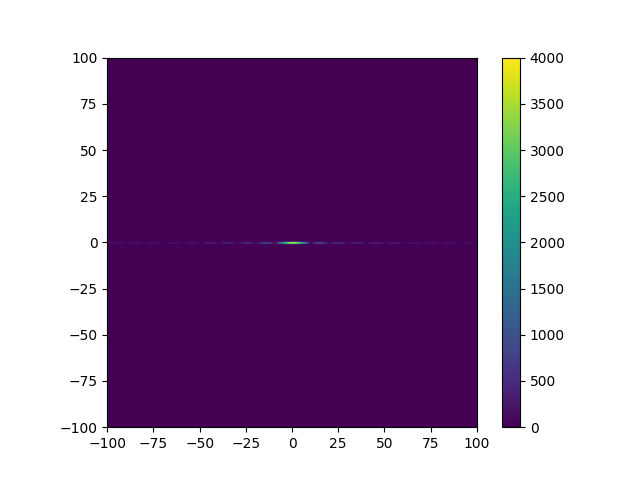
\includegraphics[width=\linewidth]{src/figures/result/ss2_amplitude_estimation.png}
		\subcaption{単スリット (幅 0.1)の回折強度パターン}\label{subfig:amplitude_sim_single2}
	\end{minipage}
	\caption{単スリットの回折強度パターンのシミュレーション}\label{fig:amplitude_sim_single}
\end{figure}

\begin{figure}[htbp]
	\begin{minipage}[ht]{0.48\hsize}\centering
		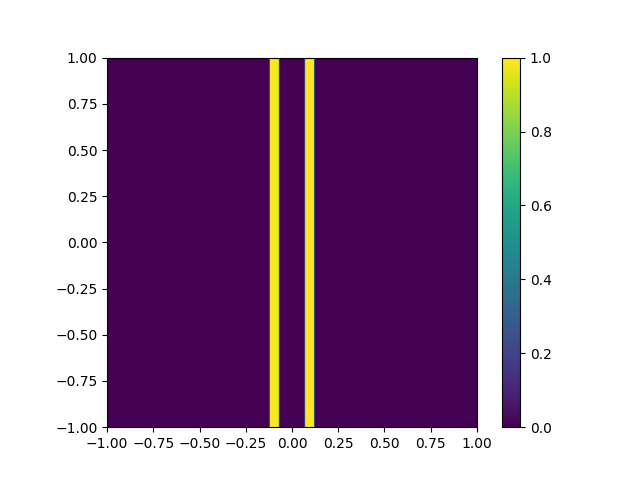
\includegraphics[width=\linewidth]{src/figures/result/ds1_original_estimation.png}
		\subcaption{二重スリット (幅 0.05, 間隔 0.1)}\label{subfig:amplitude_sim_dual1_original}
	\end{minipage}
	\begin{minipage}[ht]{0.48\hsize}\centering
		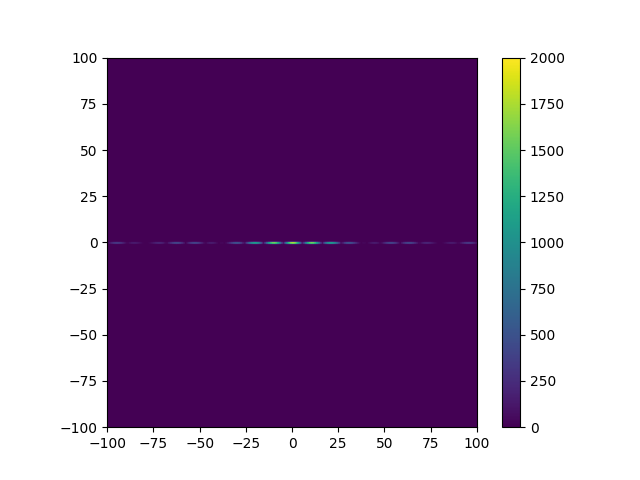
\includegraphics[width=\linewidth]{src/figures/result/ds1_amplitude_estimation.png}
		\subcaption{二重スリット (幅 0.05, 間隔 0.1)の回折強度パターン}\label{subfig:amplitude_sim_dual1}
	\end{minipage}
	\begin{minipage}[ht]{0.48\hsize}\centering
		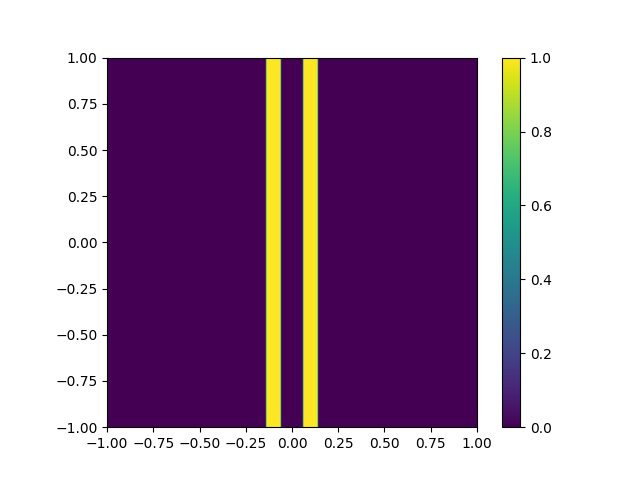
\includegraphics[width=\linewidth]{src/figures/result/ds2_original_estimation.png}
		\subcaption{二重スリット (幅 0.08, 間隔 0.1)}\label{subfig:amplitude_sim_dual2_original}
	\end{minipage}
	\begin{minipage}[ht]{0.48\hsize}\centering
		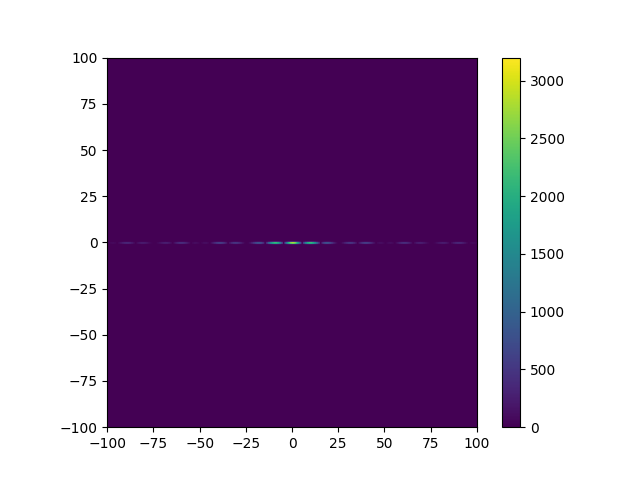
\includegraphics[width=\linewidth]{src/figures/result/ds2_amplitude_estimation.png}
		\subcaption{二重スリット (幅 0.08, 間隔 0.1)の回折強度パターン}\label{subfig:amplitude_sim_dual2}
	\end{minipage}
	\begin{minipage}[ht]{0.48\hsize}\centering
		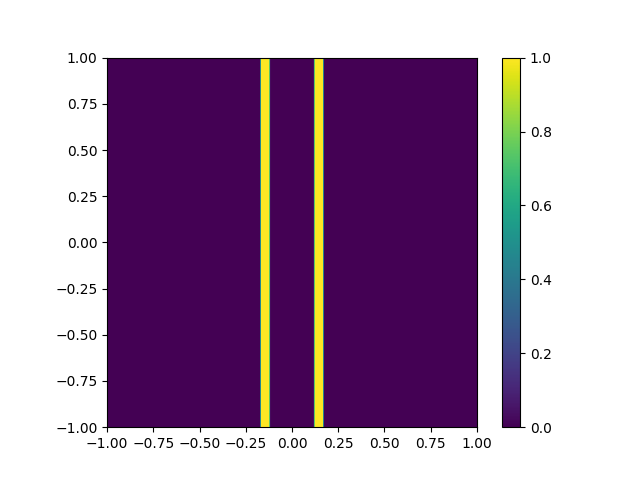
\includegraphics[width=\linewidth]{src/figures/result/ds3_original_estimation.png}
		\subcaption{二重スリット (幅 0.05, 間隔 0.15)}\label{subfig:amplitude_sim_dual3_original}
	\end{minipage}
	\begin{minipage}[ht]{0.48\hsize}\centering
		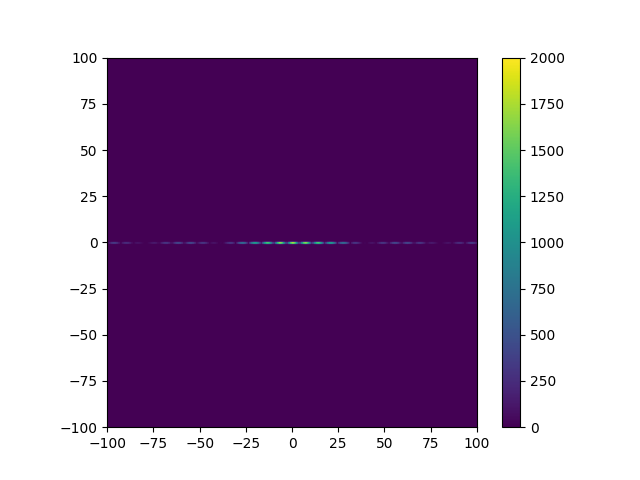
\includegraphics[width=\linewidth]{src/figures/result/ds3_amplitude_estimation.png}
		\subcaption{二重スリット (幅 0.05, 間隔 0.15)の回折強度パターン}\label{subfig:amplitude_sim_dual3}
	\end{minipage}
	\caption{単スリットの回折強度パターンのシミュレーション}\label{fig:amplitude_sim_dual}
\end{figure}
